% This is samplepaper.tex, a sample chapter demonstrating the
% LLNCS macro package for Springer Computer Science proceedings;
% Version 2.20 of 2017/10/04
%
\documentclass[runningheads]{llncs}
%
\usepackage{graphicx}
% Used for displaying a sample figure. If possible, figure files should
% be included in EPS format.
%
% If you use the hyperref package, please uncomment the following line
% to display URLs in blue roman font according to Springer's eBook style:
% \renewcommand\UrlFont{\color{blue}\rmfamily}
% For correct quotation marks (command \enquote)
\usepackage{csquotes}
% TODO: Strongly short the paper.
% TODO: Add some images. Add sensitivity analysis vs. component analysis
\begin{document}
%
\title{Interpretable Machine Learning -- A Brief History, State-Of-The-Art and Challenges\thanks{This project is funded by the Bavarian State Ministry of Science and the Arts and coordinated by the Bavarian Research Institute for Digital Transformation (bidt) and supported by the German Federal Ministry of Education and Research (BMBF) under Grant No. 01IS18036A.
The authors of this work take full responsibilities for its content.
}}
%
\titlerunning{IML - History, Methods, Challenges}
% If the paper title is too long for the running head, you can set
% an abbreviated paper title here
%
\author{Christoph Molnar\inst{1}\orcidID{0000-0003-2331-868X}}
%\and
%Second Author\inst{2,3}\orcidID{1111-2222-3333-4444} \and
%Third Author\inst{3}\orcidID{2222--3333-4444-5555}}
%
\authorrunning{Molnar}
% First names are abbreviated in the running head.
% If there are more than two authors, 'et al.' is used.
%
\institute{LMU Munich, Ludwigstr. 33, 80539 Munich, Germany
\email{christoph.molnar@gmail.com}\\
\url{https://www.slds.stat.uni-muenchen.de/people/molnar/}}
%
\maketitle              % typeset the header of the contribution
%
\begin{abstract}
  We present a brief history of interpretable machine learning (IML), give an overview of state-of-the-art interpretation methods and discuss challenges when interpreting machine learning models.
  We focus on the IML methods, putting emphasis on what interpretations can be derived mathematically and algorithmically from a machine learning model.

\keywords{Interpretable Machine Learning \and Explainable Artificial Intelligence}
\end{abstract}
%
%
Interpretability is often a deciding factor when a machine learning (ML) model is used in a product, a decision process or in research.
Interpretable machine learning (IML) methods \footnote{We will be using Interpretable Machine Learning and Explainable AI exchangeably} can be used to discover knowledge, justify the model and its predictions, control and improve models \cite{adadi2018peeking}. 
This paper reviews IML from a methodological viewpoint, with an emphasis on \textbf{what can we derive mathematically and algorithmically from an ML model}.

\section{A Brief History of IML}
A lot of IML research happened in the last couple of years.
But learning interpretable models from data has a much longer tradition.
Linear regression models have been used back in 1800 by Gauss, Legendre and Quetelet \cite{stigler1986history,legendre1805nouvelles,gauss1809theoria,quetelet1827recherches}.
Rule-based machine learning (e.g., decision rules and trees) has been an active research area since the 1980s \cite{furnkranz2012foundations}.
Both research on regression analysis and rule-based ML remain important and busy research areas to this day and are even blending together (e.g., model-based trees \cite{zeileis2008model}, RuleFit \cite{friedman2008predictive}).
Machine learning research in general also started around that time, e.g., support vector machines in 1974 \cite{vapnik1974theory}, early important work on neural networks in the 1960s \cite{schmidhuber2015deep} and boosting in 1990 \cite{schapire1990strength}.
Interpretability has always been a companion to ML.
A good example for this is the random forest, which I also see as an IML milestone for making ML practical.
Random forests, a black box machine learning model that often works well without tuning, came with a built-in feature importance measure, which contributed to its success.
The evidence that interpretability was success factor are the many citations ($>60000$ citations on Google Scholar as of September 2020) of the original paper \cite{breiman2001random}, but also of papers improving the importance measure (\cite{strobl2008conditional,strobl2007bias,hapfelmeier2014new,ishwaran2007variable}).
In the 2010s came the deep learning hype, after a deep neural network won the ImageNet challenge.
A few years after that, the IML field really took off (around 2015), judging by frequency of the search terms "Interpretable Machine Learning" and "Explainable AI" on Google (Figure \ref{fig:count} right)and papers published with these terms (Figure \ref{fig:count} left).
\begin{figure}
  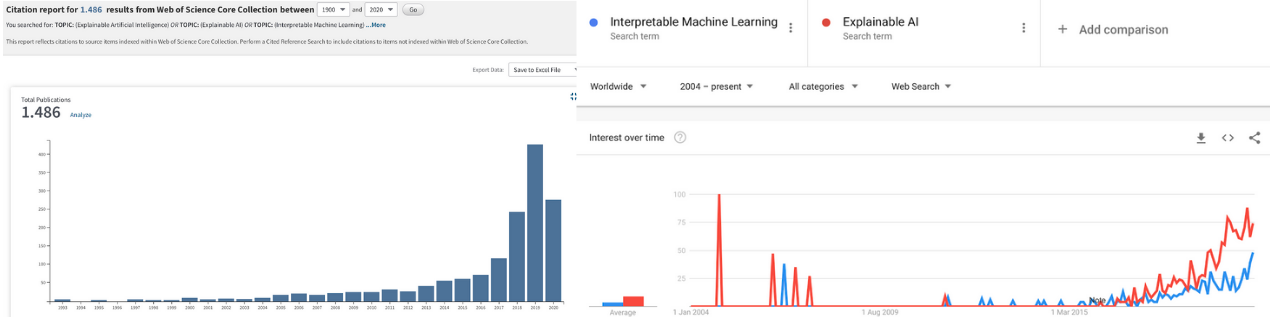
\includegraphics[width=\textwidth]{citation-search.png}
  \caption{Left, Right}
  \label{fig:count}
\end{figure}
Since then, many approaches have been introduced to the field, many of them model-agnostic explanation methods, i.e., working for different types of ML models, but also model-specific explanation methods to interpret, e.g., deep neural networks and tree ensembles.
Rule-based ML and statistical regression models continue to be developed and serves both as full ML models, but also as building blocks for many of the newer IML approaches.
%Could it be that only the terms have changed, but the field has always been there and the same?
%I would still argue that the field has reached a new form, as evidenced by new keywords "Interpretable Machine Learning" and "Explainable Artificial Intelligence", but also by bringing in new ideas from other fields, pulling many unconnected research fields together and an additional focus on model-agnostic ML interpretation methods.
% TODO: Find more evaluation papers
\textbf{Today} IML reached a first state of usability.
Some methods have been established with a better understanding of weaknesses and strengths.
There are dozens of surveys of the IML field \cite{molnar2019,guidotti2018survey,vilone2020explainable,rosenfeld2019explainability,adadi2018peeking,anjomshoae2019explainable,du2019techniques,carvalho2019machine}.
The field is starting to further consolidate terms and knowledge \cite{hall2019systematic,doshi2017towards,murdoch2019definitions,samek2019towards,preece2018stakeholders} and we have some ideas how to evaluate explanations and interpretability methods \cite{mohseni2018multidisciplinary}.
Many open source software packages implement various techniques \cite{iml,biecek2018dalex,pedregosa2011scikit,klaise2020alibi,nori2019interpretml} .
These software tools give ML practitioners the means to interpret their models.
Regulation such as GDPR has spurred a discussion around further needs of interpretability \cite{wachter2017counterfactual}.
IML has also arrived in industry \cite{gade2019explainable}, there are startups that focus on machine learning interpretability and also big tech companies offer software \cite{exler2019if,arya2020ai,hall2017machine}.

\section{IML Methods}

In this section we broadly cover some popular IML methods.
We distinguish IML methods between component and sensitivity analysis\footnote{Not to be confused with the research field of sensitivity analysis, which studies the uncertainty of outputs in mathematical models and systems. There are methodological overlaps (e.g., Shapley values), but also differences in methods and how input data distributions are handled}.
An IML method that works by component analysis assigns meaning to \textit{(learned) model parameters and structures} while sensitivity analysis \textit{probes the model with artificial data points and describes its behavior}.\footnote{Some surveys \cite{vilone2020explainable,guidotti2018survey,du2019techniques} divide methods into \textit{ante-hoc (alternatively: transparent design, white box models)} and \textit{post-hoc} IML method, depending on whether interpretability is considered at model design and training or after training, leaving the (black-box) model unchanged. Another category divides model-agnostic and model-specific. Component vs. sensitivity analysis is, in our opinion, another interesting view and why only repeat what others already have said?}
The idea of component analysis is closely related to decomposability:
You can only analyze components of a model that can be decomposed into individual components that we can interpret individually, like weights in a linear model.
Component analysis does not necessarily require that the user understands the model in its entirety (simulatability), but only individual parts.
Component analysis is always model-specific, e.g., a linear regression model can be interpreted by analyzing its coefficients, while a decision tree can be interpreted by visualizing the learned decision structure.
Sensitivity analysis is mostly model-agnostic and works by manipulating input data and analyzing the respective model predictions.
Usually, we analyze the components of ML models that are said to be inherently interpretable, but there are also ways to analyze components of more complex models, but this often requires more work.
\textit{Inherently interpretable models} are models with learned structures and learned parameters which can be assigned some meaning.
Linear regression models, decision trees and decision rules are considered to be interpretable \cite{freitas2014comprehensible,huysmans2011empirical}.
%As a rule of thumb for when we do an introspection is that we are not probing the model with various (manipulated data points).
Linear regression models ($Y = \beta_0 + \beta_1 x_1 + \ldots + \beta_p x_p$) can be interpreted by analyzing components:
The model structure, a weighted sum of features, allows that we interpret the $\beta$-weights as the effect that a feature has on the prediction.
Many extensions exist \cite{hastie1990generalized,fahrmeir2013multivariate,gelman2006data} and linear regression models remain an active field of research \cite{fasiolo2020scalable,caruana2015intelligible,fasiolo2020fast,ustun2016supersparse} 
Decision trees and other rule-based ML models have a learned structure (e.g.,\enquote{IF feature $x_1 > 0$ and feature $x_2 \in \{A,B\}$, THEN predict 0.6}).
We can interpret the learned structure to trace how the model makes predictions.
Rule-based ML also remains an active area of research (for example, \cite{wang2015falling,letham2015interpretable,hothorn2015ctree}).

The more complex interpretable models get (e.g., linear models with hundreds of features and complex interaction terms or deep decision trees), the more difficult the interpretation becomes.

Component analysis is how we interpret inherently interpretable models, but component analysis can be used to explain black box models.
For example, the abstract features learned by a deep convolutional neural network (CNN) can be visualized by finding or generating images that activate a feature map of the CNN \cite{olah2017feature}.
% TODO: Add image
Feature visualization showed that CNNs learn low-level features such as edge-detectors at the early neural layers and gradually more abstract detectors for textures and objects in higher layers.
As one other example among many, there are various feature importance measures for the random forest that are based on analyzing components.
For example, the minimal depth distribution \cite{randomForestExplainer,ishwaran2010high} and the Gini importance \cite{breiman2001random} analyze the structure of the trees of the forest.
.
Since all IML methods that rely on component analysis are model-specific, the explanations are tied to that ML model.
If a different ML model is used, the IML method has to change, which is a disadvantage.
But if a model is well understood and frequently used in community, like random forest in ecology research \cite{cutler2007random}, model component analysis can be a powerful tool.
Component analysis can explain the overall model behavior (global) or individual predictions (local).
In many cases the components of a model has the same global and local interpretation.
For example, in linear regression models the weights explain both how the features affect an individual prediction, but also summarize the global behavior.


\paragraph{IML method based on sensitivity analysis} often treat the ML model as a closed system that receives an input and produces an output, the prediction.
We further distinguish between local and global explanations that sensitivity based IML methods can produce.

\paragraph{Local explanations} are used to explain individual predictions of an ML model.
Local explanation methods have received much attention and there has been a lot of innovation in the last years.
Popular local IML methods are LIME \cite{ribeiro2016should}, Shapley Values \cite{lundberg2017unified,vstrumbelj2014explaining} and Counterfactual Explanations \cite{wachter2017counterfactual,dandl2020multi}.
Counterfactual explanations explain predictions in the form of what-if scenarios, which builds on a rich tradition in philosophy.
According to findings in the social sciences \cite{miller2019explanation}, counterfactual explanations are \enquote{good} explanations because they are contrastive and focus on a few reasons.
A different approach originates from collaborative game theory:
The Shapley values \cite{shapley1953value} provide an answer on how to fairly share a payout among the players of a collaborative game.
The collaborative game idea can be applied to ML \cite{vstrumbelj2014explaining,lundberg2017unified,lundberg2018consistent}: The predicted value is the payout, each feature value is a player.
Another popular method are local interpretable model-agnostic explanations, short LIME \cite{ribeiro2016should}.
LIME uses surrogate models, i.e., the method trains an interpretable model such as a linear regression model to approximate the predictions of original ML model.
Numerous extensions of LIME exist, that try to fix issues with the original method, extend it to other tasks and data or analyze its properties \cite{hu2018locally,rabold2018explaining,rabold2019enriching,visani2020optilime,haunschmid2020audiolime,rahnama2019study,shankaranarayana2019alime}.
% TODO: Add the many extensions of Shapley Values
Some IML methods rely on model-specific knowledge to analyze how changes in the input features changes the output.
Saliency maps for CNNs make use of the network gradients to explain individual classifications.
The explanations are in the form of heatmaps that show how changing a pixel can change the classificaiton.
The saliency map methods differ in how they backpropagate \cite{sundararajan2017axiomatic,lundberg2017unified,montavon2017explaining,simonyan2013deep,shrikumar2016not}.
Additionally model-agnostic versions \cite{ribeiro2016should,lundberg2017unified,zeiler2014visualizing} exist for analyzing image classifiers.

\paragraph{Global, model-agnostic explanation methods} are used to explain how the model behaves on average for some given dataset.
A useful distinction of global explanations are feature importance and feature effect.
Feature importance ranks features based on how relevant they were for the prediction.
Permutation Feature Importance \cite{fisher2019all}, which is based on permuting features is a popular importance measure, originally suggested for random forests \cite{breiman2001random}, now available as model-agnostic version.
An alternative are variance based measures.
See \cite{wei2015variable} for an overview of all the ways to measure importance.
The feature effect expresses how a change in a feature changes the predicted outcome.
Popular feature effect plots are Partial Dependence Plots \cite{friedman2001greedy}, Individual Conditional Expectation Plots \cite{goldstein2015peeking} and Accumulated Local Effect  (ALE)  Plots \cite{apley2016visualizing}.

\paragraph{Surrogate models}\footnote{Surrogate models are related to knowledge distillation and the teacher-student model.} are interpretable models designed to \enquote{copy} the behavior of the ML model.
They do not neatly fit into the categorization of component or sensitivity analysis, as they combine both:
The surrogate approach treats the ML model as a black box, only requiring the input / output data  (similar to sensitivity analysis), but the interpretation is based on analyzing components of the interpretable surrogate model.
Many methods are surrogate model approaches \cite{puri2017magix,molnar2019,ming2018rulematrix,ribeiro2016should,frosst2017distilling,bastani2017interpreting,craven1996extracting,krishnan2017palm}.
They differ in which ML model they can be used for, the data sampling strategy, the interpretable model that is used and so on.
There are also methods for extracting, e.g., decision rules from specific models based on their internal components such as weights \cite{andrews1995survey,augasta2012rule}, which resembles more the component analysis approach.

% TODO: Add that sensitivity analysis can also be used for inherently interpreteable models

%What I missed out on:
%
%- Human-Computer Interaction, e.g. (Explainable Artificial Intelligence: a Systematic Review) sees Explainable AI as the intersection between Artificial Intelligence and Human-Computer Interaction.
%- Ethics and Philosophy.
%- Explanations can have different \textit{structure}: text, image, tables, ...
%- Methods that are model-agnostic might not be input data agnostic, e.g., PDP does not make sense for pixel data as used in image classification
%- Some methods are designed or adapted so that we can more easily understand what its components do. For example for neural networks we can \textit{disentangle} the individual neurons TODO:CITE, so that we can interpret them better.
%- TODO: Add more to the idea of making components of a (black-box) ML model more interpretable. This can be e.g. tree pruning, adding sparsity to linear regression models, disentangle neurons.
%- We can use sensitivity analysis also to interpretable models
%- We did not touch topics where data is analyzed before modelling to understand the data better
%- Idea that we can decompose the function with functional ANOVA and so on

%\paragraph{Blending all together.} This list was not exhaustive. For example, there are also ways to add interpretability constraints to a model, such as monotonicity or sparsity.
%This can helps component analysis, e.g., a linear model with most coefficients at zero is easier to interpret.
%But this can also help with sensitivity analysis, as PDPs of monotonic features will only show in one direction.

\section{Challenges}

This is an incomplete list of some of the challenges of IML, mostly based on \cite{molnar2020pitfalls}.

\paragraph{Statistical Uncertainty and Inference}
Many IML methods such as permutation feature importance or Shapley values provide explanations without quantifying the uncertainty of that explanation.
The the model itself, but also the explanations are usually computed from data and are subject to variance.
We have to become more rigorous in reporting both reporting the explanations, but also their uncertainty.
Some research is working towards the goal of quantifying uncertainty of explanations, for example for feature importance \cite{watson2019testing,fisher2019all}, layer-wise relevance propagation \cite{fabi2020feature} and Shapley values \cite{williamson2020efficient}.
Quantifying uncertainty and expressing it as error bars, confidence intervals or also test statistics and p-values is an important part of statistical modeling.
The goal of statistical inference is to infer properties of the underlying data distribution of the phenomenon that is being studied.
In this process, a statistical model is proposed with a set of assumptions (for example, a linear model with assumptions that the features only have additive effects).
When all assumptions are met, the statistical model may be interpreted to reflect the true data generating process.
Statistical modeling is used for testing scientific hypothesis.
Machine learning modeling takes a different approach:
Instead of assuming a model of the data generating process, various flexible models are compared on test data.
It is desirable to draw also conclusions from these models about the underlying data generating process.
With IML, with have method to compute meaningful properties of the model. 
But to infer properties about the data generating process from the ML model, we have to specify the assumptions needed that allow a combination of ML model and IML method to be interpreted as the \enquote{true} model.
We also need tools and procedures to check these assumptions.
Hopefully we can avoid problems in statistical testing, such as p-hacking \cite{head2015extent} and the resulting publication bias \cite{begg1994publication}.

\paragraph{Causal interpretation.}
Ideally, a model relies on the true causes to make a prediction.
Then we could  interpret it causally, making statements about the underlying phenomena, which is the focus of ML in research, but also makes models robust against adversarial attacks, and more useful when used as a basis for decision making.
Unfortunately, predictive performance and causality can be conflicting goals.
For example, today's weather directly causes tomorrow's weather, but we might only have access to feature \enquote{wet ground}.
Using \enquote{wet ground} in the prediction model for \enquote{tomorrow's weather} is useful as it has information about \enquote{today's weather}, but we are not allowed to interpret it causally, because the confounder \enquote{today's weather} is missing.
Further research is needed to understand when we are allowed to make causal interpretations of an ML model.
First steps have been made for permutation feature importance \cite{konig2020relative} and Shapley values \cite{ma2020predictive}.

\paragraph{Lack of definition} is a common critique of the field \cite{lipton2018mythos,doshi2017towards}.
Without a definition of "interpretability", how can we decide if a new method explains ML models better?
To evaluate the \textbf{predictive performance} of an ML model, we simply compute the prediction error on test data given the groundtruth label.
To evaluate the \textbf{interpretability} of that same ML model is not as easy.
We do not know what the groundtruth explanation looks like and have no straightforward mean to quantify how interpretable a model is or how correct an explanation is.
Instead of having one groundtruth explanation, various \textbf{quantifiable aspects of interpretability} are emerging \cite{poursabzi2018manipulating,philipp2018measuring,molnar2019quantifying,hauenstein2018computing,zhou2018measuring,akaike1998information,schwarz1978estimating,poursabzi2018manipulating,dhurandhar2017tip,friedler2019assessing}.

Two main ways of evaluation of interpretability have emerged: \textit{objective evaluations} which are mathematically quantifiable metrics, and {human-centered evaluations} which involve studies with users.
It seems like we are on our way to have many definitions of \textit{various aspects} of interpretability such as sparsity, interaction strength, fidelity (how well explanation approximates the ML model), sensitivity to perturbations,  and a user's ability to run a model on a given input (simulatability) are examples of such aspects.
The challenge ahead remains to establish a best practice on how to evaluate interpretation methods and the explanations they produce.
Here we should also look to the field of Human-Computer Interaction who do exactly that.

We have focused mostly on the methodological, mathematical challenges in a rather static setting, where you are given a machine learning model and data.
\textit{Many more} challenges lie ahead to improve interpretability of machine learning.
What is the best way to explain a machine learning model for people with a specific background and how do we present the explanations?
How are people affected by explanations, how are explanations maybe misused (CITE fairwashing by HIma)?
This is also a rather static view point in the sense that we can do a lot if we allow a more interactive way of modeling and "having a conversation" between a person and the model or even the modeling process.
How do we present multiple maybe conflicting explanations, e.g., when you generate multiple counterfactual explanations?

\section{Discussion}

Interpretable Machine Learning is a young field, but has deeper roots in Statistics and Computer Science and also draws from other fields such as the social sciences, human-computer interaction and game theory.
There has been Cambrian explosion of methods in the 2010s, including model-agnostic interpretation methods and many specialized methods for, e.g., deep neural networks.
Many of these methods have found their way into open source software and products of startups and tech companies.
Interpretable Machine Learning is used in science, company products and processes.
While we have reached a first maturity, there a still some challenges ahead, such as feature dependence, causality and inference.
Many IML methods are imported from other fields, so thinking outside the box (pun intended) might help in the challenges ahead.
We believe that the field has to reach out horizontally -- to other domains -- and vertically -- drawing from the rich research in statistics and computer science.


%
% ---- Bibliography ----
%
% BibTeX users should specify bibliography style 'splncs04'.
% References will then be sorted and formatted in the correct style.
%
% \bibliography{mybibliography}
%

\vskip 0.2in
\bibliographystyle{splncs04}
\bibliography{Bib}

\end{document}
